\chapter{Code changes in the \ac{KIEM}}
\label{chapter:KiemChanges}
Although the project attempts to realize most of the objectives without
changing the \ac{KIEM} itself some changes were necessary.
This mostly involves adding new methods to the \ac{API} in order to
gain access to previously hidden properties.

Also some changes had to performed where properties were loaded from hard
coded default values. These were changed so that the hard coded default is
only used if the \ac{KIEMConfig} plug-in is not registered to supply previously
saved properties.

However all changes that were made to the \ac{KIEM} plug-in were merely additions
and shouldn't break any plug-ins relying on the old implementation.

% generated by KIEM
% required packages: 
% \usepackage{multicol}
% \usepackage{multirow}
\begin{tabular}{| l | l | l | p{1.2cm} | l | l | } \hline
\multicolumn{4}{|c|}{}
 & \multicolumn{2}{c|}{Test Component}
\\ \hline
Model file & Iteration & Status & Finished on step & Iteration & Step finished \\ \hline
\multirow{4}{*}{/test/default.kids} & 0 & Done & 7 & 0 & 7 \\ 
 & 1 & Done & 7 & 1 & 7 \\ 
 & 2 & Failed & 2 & 2 & 2 \\ 
 & 3 & Done & 7 & 3 & 7 \\ 
\hline
\multirow{4}{*}{/test/test.strl} & 0 & Done & 7 & 0 & 7 \\ 
 & 1 & Done & 7 & 1 & 7 \\ 
 & 2 & Failed & 2 & 2 & 2 \\ 
 & 3 & Done & 7 & 3 & 7 \\ 
\hline
\label{figure:autoTest[test]Output}
\end{tabular}

% generated by KIEM
% required packages: 
% \usepackage{multicol}
% \usepackage{multirow}
\begin{tabular}{| l | l | l | p{1.2cm} | l | l | } \hline
\multicolumn{4}{|c|}{}
 & \multicolumn{2}{c|}{Test Component}
\\ \hline
Model file & Iteration & Status & Finished on step & Iteration & Step finished \\ \hline
\multirow{4}{*}{/test/default.kids} & 0 & Done & 7 & 0 & 7 \\ 
 & 1 & Done & 7 & 1 & 7 \\ 
 & 2 & Failed & 2 & 2 & 2 \\ 
 & 3 & Done & 7 & 3 & 7 \\ 
\hline
\multirow{4}{*}{/test/test.strl} & 0 & Done & 7 & 0 & 7 \\ 
 & 1 & Done & 7 & 1 & 7 \\ 
 & 2 & Failed & 2 & 2 & 2 \\ 
 & 3 & Done & 7 & 3 & 7 \\ 
\hline
\label{figure:autoTest2[test]Output}
\end{tabular}
\section{Schema files and Interfaces}
\index{Extension point}
In order to provide additional functionality for other plug-ins we choose the extension
point mechanism described in section \ref{section:ConfTechnologyExtension}. This is done
is order to retain the old functionality of the plug-in while on the other hand giving
options to ask extending plug-ins for their contributions. 

The extension points described in greater detail in the next sections consist
of a schema file for defining the extension point and an interface that contains the 
methods that extending components have to supply.

\subsection{Toolbar Contribution Provider}
\label{section:ToolbarContributionProvider}
\index{Toolbar Contribution Provider}
The purpose of the toolbar contribution provider is to allow other plug-ins to put
items onto the toolbar. 
There are two reasons for using the extension point mechanism
rather than making the toolbar available and have other plug-ins put their
contributions directly on it:
\begin{enumerate}
 \item At the moment the toolbar and all contributions are created programatically. Switching
the entire native toolbar of the Execution Manager to adding the actions to the toolbar
through the org.eclipse.ui.toolbar extension point would require major code changes.
 \item A programatic approach gives control over the contributions to the Execution Manager.
This means that the order of the native Execution Manager buttons is always the same and in the
same place. It also means that the Execution Manager can choose to ignore contributions if the
toolbar gets too crowded.
\end{enumerate}
\begin{figure}[IToolbarContributor]
  \centering
  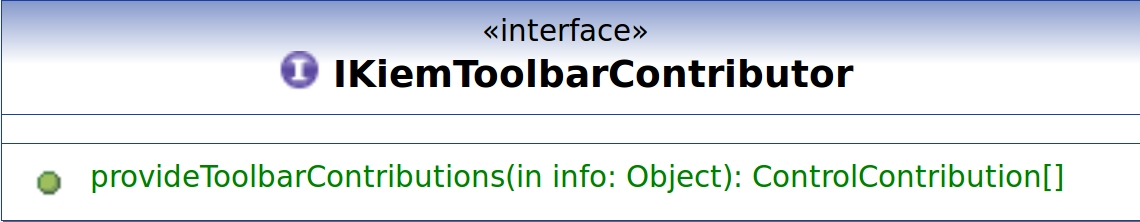
\includegraphics[scale=.3]{IKiemToolbarContributor.jpg}
  \caption[The interface for Toolbar Contribution Providers]%
  {The interface for Toolbar Contribution Providers\protect\footnotemark}
  \label{fig:IToolbarContributor}
\end{figure}

The schema file for components that want to add contributions to the toolbar is quite simple.
It only requires them to implement the interface shown in figure \ref{fig:IToolbarContributor}.
The implementing class provides an array with all ControlContributions they want to add to the toolbar.
A ControlContribution for a toolbar can be almost any swt.Widget like Labels, Buttons, Comboboxes, ....

When the Execution Manager starts to build the views toolbar it will start by asking the contributors
for their contributions, add them to the toolbar and then adds its own elements. This causes
the toolbar to have the native elements always in the same order.
The contributed elements will be added from left to right in the order that they are in the array. However there
is no guarantee on the order in which the extending plug-ins are asked.
Figure \ref{fig:ToolbarWithContributions} shows the Execution Manager toolbar with the two combo boxes belonging to \ac{KIEMConfig}
contributed through the extension point. Figure \ref{fig:ToolbarWithoutContributions} shows the same toolbar without
the contributions.
\begin{figure}[ToolbarWithContributions]
  \centering
  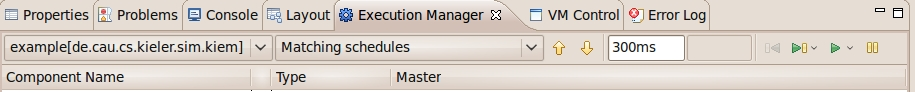
\includegraphics[scale=.4]{ToolbarWithContributions.jpg}
  \caption[The Execution Managers Toolbar with two contributed Comboboxes]%
  {The Execution Managers Toolbar with two contributed Comboboxes\protect\footnotemark}
  \label{fig:ToolbarWithContributions}
\end{figure}
\begin{figure}[ToolbarWithoutContributions]
  \centering
  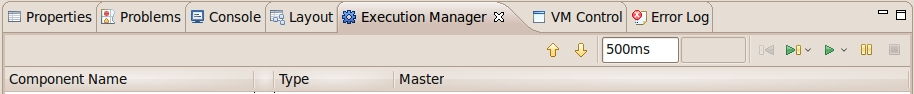
\includegraphics[scale=.4]{ToolbarWithoutContributions.jpg}
  \caption[The Execution Managers Toolbar without contributions]%
  {The Execution Managers Toolbar without contributions\protect\footnotemark}
  \label{fig:ToolbarWithoutContributions}
\end{figure}

%\begin{itemize}
% \item asks registered plugins for list of control contributions
% \item add items to toolbar
% \item KIEM native items stay in same position
%\end{itemize}

\subsection{Configuration provider}
\label{section:ConfigurationProvider}
\index{Configuration Provider}
The purpose of the configuration provider is to allow internal attributes of the
Execution Manager to be stored in another plugin. 

This is done through an extension point to allow any plug-in to listen to changes
in the Execution Manager's attributes. It also means that there may be multiple
plug-ins that provide values for properties and not all plug-ins may have the value for
a property needed by the Execution Manager. Through the plug-in mechanism the \ac{KIEM}
can ask all providers for values and choose the one he would like to use.

\begin{figure}[Configuration Provider Interface]
  \centering
  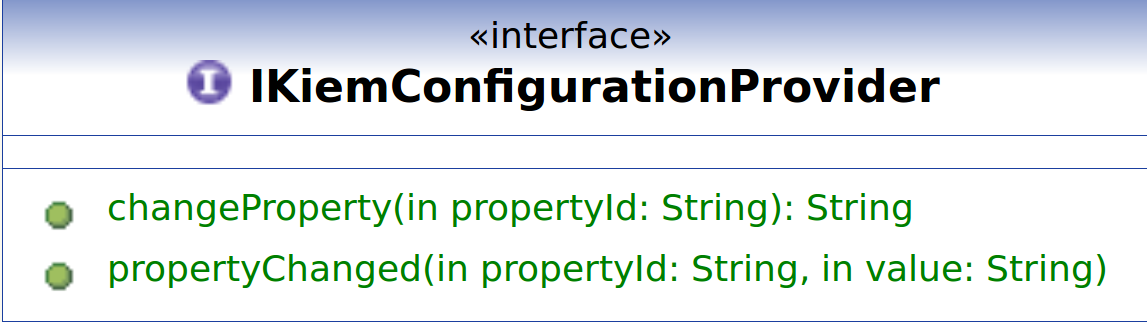
\includegraphics[scale=0.3]{IKiemConfigurationProvider.png}
  \caption[The Interface of the Configuration Provider]%
  {The Interface of the Configuration Provider\protect\footnotemark}
  \label{fig:UMLConfigurationProvider}
\end{figure}

The two methods from the interface shown in Figure \ref{fig:UMLConfigurationProvider} work
in the following way:



%\begin{itemize}
% \item notify of current configuration changes (aimed step duration text field)
% \item ask providers for saved preferences
% \item can ask any key/value
% \item limited to String due to preference store
%\end{itemize}

\subsection{Event Manager}
The main purpose of the Event Manager is to inform DataComponents of events
happening in the \ac{KIEM} during execution. This behavior has been modified to include 
events that happen while the execution is not running. This modification lead to the 
creation of another extension point in order to allow other plug-ins to be notified
on any of these events as well. The classes implementing the interface 
(see figure \ref{fig:UMLEventListener}) required by this extension point will be notified
on any event that happens inside the \ac{KIEM}.

\begin{figure}[Event Listener Interface]
  \centering
  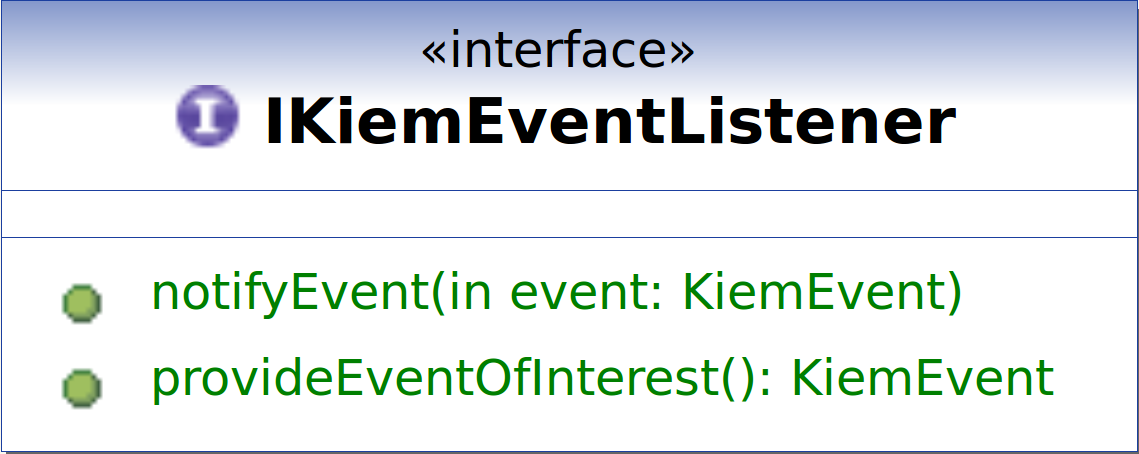
\includegraphics[scale=0.3]{IKiemEventListener.png}
  \caption[The Interface of the Event Listener]%
  {The Interface of the Event Listener\protect\footnotemark}
  \label{fig:UMLEventListener}
\end{figure}

The semantics of the methods will be explained in detail in the following two subsections.

\subsubsection*{provideEventOfInterest()}
This method is directly derived from the method with the same name in the AbstractDataComponent class
of the \ac{KIEM} plug-in. It is called by the EventManager to determine which events the implementing
class is interested in. This is done to improve effiency and not flooding components with events
they are not interested in.

Based on the response the EventManager puts the component into lists along with the DataComponentWrappers
already inside.
\subsubsection*{notifyEvent(KiemEvent event)}
This method is called by the EventManager when something happens inside the \ac{KIEM} that the implementing
classes might be interested in.


%\begin{itemize}
% \item notify plugins of events happening in KIEM
% \item may be any event and carry information
% \item currently used for file event, IPath as information
%\end{itemize}

\section{KIEMPlugin.java}
The main Activator class contains almost the entire \ac{API} of the \ac{KIEM}.
Therefore any additions to that has to performed in this class which means that
most of the adjustments were made here.


\begin{enumerate}
 \item A couple of methods were added to inform the listeners registered through
the ConfigurationProvider extension point of changes the user made through the \ac{UI} of the \ac{KIEM}.
 \item The method that takes care of loading an execution file was split. This was done to allow
other plug-ins to pass an IPath object directly to the method and perform a load of that file without
having to go through the \ac{UI}. This method was also shifted around a little in order to detect
missing execution files before the load enters the UIThread. This was necessary to make is possible for
the callers of the method to catch the resulting exception.
Another modification was that the method has to be able to process files that are not in the currently
running workspace but were added through an extension point.
 \item getter for configuration elements
 \item relay to KiemView to trigger updates
\end{enumerate}

\section{KIEMView}
\begin{itemize}
 \item changes to toolbar creation
 \item provide means to set view as dirty when changes happen
 \item refresh method to reload values, not needed before because no change except by user
\end{itemize}